% !TeX root = RJwrapper.tex
\title{stplanr: A Package for Transport Planning}
\author{by Robin Lovelace, Richard Ellison}

\maketitle

\abstract{%
Tools for transport planning should be flexible, scalable and transparent (open source).
The \textbf{stplanr} package demonstrates and provides a home for such tools, with an emphasis on spatial transport data and non-motorized modes.
\textbf{stplanr} facilitates some common transport planning tasks including:
downloading and cleaning transport datasets;
creating geographic `desire lines' from origin-destination (OD) data;
route assignment, via the \code{SpatialLinesNetwork} class and
interfaces to routing services such as CycleStreets.net;
calculation of route segment attributes such as bearing and aggregate flow;
and `travel watershed' analysis.
This paper demonstrates this functionality using reproducible examples on real transport
datasets.
More broadly, the experience shows open source software can form the basis of a reproducible
transport planning workflow.
\textbf{stplanr}, alongside other packages and open source projects,
could provide a more transparent and democratically accountable alternative to the
current approach which is heavily reliant on proprietary and technically and financially inaccessible software.
}

\section{Introduction}\label{introduction}

The practice of transport planning can been defined as
"preparing, assessing and implementing policies, plans and projects to
improve and manage our transport systems"
\citep{jones_road_2014}.
This inevitably involves judgments based on intuition, experience and political considerations.
However, with the push for evidence-based policy, the pressure to adopt scientific methods has grown.
This includes the development and use of open source software \citep{balmer_matsim-t:_2009}.
Transport planning is a diverse field with diverse software requirements \citep{boyce_forecasting_2015}, but the following generalisations can be made.
Software for transport planning should be:

\begin{itemize}
\tightlist
\item
  flexible, able to handle a wide range of data formats
\item
  scalable, able to work at multiple geographic levels from single streets to large cities and regions
\item
  robust and reliable, tested on a range of datasets and able to work 'out of the box' in a range of real-world projects.
\item
  open source and reproducible. This ensures transparency and encourages citizen science and evidence-based, democratic decision making based in which many people can participate in the technical discussion and analysis.
\end{itemize}

This paper sets out to demonstrate, with reproducible examples, that open source software with a command-line interface (CLI) can provide a foundation for transport planning software that meets
each of these criteria.
We argue that R provides a strong basis for progress in this direction, as it contains many of the building blocks for a transport planning workflow.
Packages such as \CRANpkg{sp}
\citep{pebesma_classes_2005} and \CRANpkg{rgeos}
\citep{bivand_rgeos:_2016} greatly extend R's spatial data handling and
modelling capabilities \citep{bivand_applied_2013}
(see the \ctv{Spatial} task view for an overview).
Packages building on
spatial class system have been developed for specific domains,
including: disease mapping and modelling, with packages such as \CRANpkg{SpatialEpi} and \CRANpkg{diseasemapping} \citep{kim_spatialepi:_2016,brown_diseasemapping:_2016}; spatial ecology, with the \textbf{adehabitat} family of packages \citep{calenge_package_2006};
and visualisation, with packages such as \CRANpkg{leaflet}, \CRANpkg{tmap}, \CRANpkg{mapview} and \CRANpkg{mapmisc} \citep{RJ-2016-005}.
However, there has been little prior work to develop R functionality designed
specifically for transport planning, with the notable exceptions of
\href{http://r-forge.r-project.org/projects/travelr/}{TravelR} (a package on R-Forge last updated in 2012)
and \href{https://github.com/ropensci/gtfsr}{gtfsr}
(a package for handling  General Transit Feed Specification (GTFS) data).

Inspired by such efforts and driven by our own research needs, the
primary aim of \textbf{stplanr} is to provide an R toolbox for transport planning, with an emphasis on spatial data and active modes.
The workflow demonstrated in this package is intended to be part of the wider process of transport planning, which is undergoing a paradigm shift towards sustainability \citep{banister_sustainable_2008} and `Big Data' \citep{zheng_big_2016}.
% Although the focus is on spatial transport datasets
% (and most transport problems contain a spatial component),
% \textbf{stplanr} could be extended in non-spatial directions such as mode
% choice modelling.

\subsection{Motivations}\label{motivations}

The relative lack of R packages for transport applications
(compared with other disciplines such as epidemiology
and ecology) is surprising.
Transport
problems are ubiquitous,\footnote{Most people can identify interventions that they
  think would make the transport systems they interact with more
  sustainable. Think about the paths and roads you travel on, for
  example: what interventions would you prioritise to improve
  non-motorised access, for walking, cycling and wheel-chairs? What
  quantitative evidence would you need to communicate this to the
  relevant authorities?}; R is proficient at handling transport data
(including spatial and travel survey data);
and R is increasingly used in
in applied domains \citep{jalal_overview_2017,moore_why_2017}
and within public and private organisations that generate and use transport data.
Despite the growth in open access datasets and open source software, transport planning is still inaccessible to most people.
In this context \textbf{stplanr} was motivated by the need to reduce the barriers of access to data-driven transport planning, financial and technical, through open source software.
R is an established open source project with a large user community that already provides many tools that could be useful in transport planning.
The paper is therefore not only about showcasing new tools within \textbf{stplanr} but also about demonstrating how \emph{existing} tools in R can be used for transport planning.

\textbf{stplanr} cannot cover all bases in Transport Planning and it is hoped that the ideas, functions and datasets described in this paper inspire
parallel developments in the space of `R for transport applications'.
By making the package title deliberately broad in its scope, we plan to expand
\textbf{stplanr}'s functionality over time
to help build community of R-using
transport researchers. We welcome feature requests and feedback at the
package's \href{https://github.com/ropensci/stplanr/issues}{online
home}.

R is already used in transport applications, as illustrated by recent
research that applies packages from other domains to transport problems.
For instance, \citeauthor{efthymiou_use_2012}
(\citeyear{efthymiou_use_2012}) use R to analyse the data collected from
an online survey focused on car-sharing, bicycle-sharing and electric
vehicles. \citeauthor{efthymiou_use_2012}
(\citeyear{efthymiou_use_2012}) also used R to collect and analyse
transport-related data from Twitter using packages including
\CRANpkg{XML}, \CRANpkg{twitteR} and \CRANpkg{ggplot2}. These packages
were used to download, parse and plot the Twitter data using a method
that can be repeated and the results reproduced or updated. More general
statistical analyses have also been conducted on transport-related
datasets using packages including \CRANpkg{muStat} and \CRANpkg{mgcv}
\citep{diana_studying_2012,cerin_walking_2013}. Despite the rising use
of R for transport research, there has yet been to be a package for
transport planning.

The design of the R language, with its emphasis on flexibility, data
processing and statistical modelling, suggests it can provide a powerful
environment for transport planning research. There are many quantitative
methods in transport planning, many of which fit into the
classic `four stage' transport model which involves the following steps
\citep{willumsen_modelling_2011}:
(1) trip \emph{generation} to estimate trip freqency from origins;
(2) \emph{distribution} of trips to destinations;
(3) \emph{modal split} of trips between walking, cycling, buses etc.;
(4) \emph{assignment} of trips to the transport route network.
To this we would like to add two more stages for the big data age:
(0) data processing and exploration; and
(5) validation.
This sequence is not the only way of transport modelling
and some have argued that its dominance has reduced innovation.
However it is certainly a common approach and provides a useful
schema for classifying the kinds of task that \textbf{stplanr} can tackle:

\begin{itemize}
\tightlist
\item
  Accessing and processing of data on transport infrastructure and
  behaviour (stage 0)
\item
  Analysis and visualisation of the transport network (0)
\item
  Analysis of origin-destination (OD) data and the visualisation of
  resulting `desire lines'
\item
  The allocation of desire lines to roads and other guideways via
  routing algorithms to show commonly used routes through geographical
  space
\item
  The aggregation of routes to estimate total levels of flow on segments
  throughout the transport network
\item
  Development of models to estimate transport behaviour currently and
  under various scenarios of change
\item
  The calculation of `catchment areas' affected by transport
  infrastructure
\end{itemize}

The automation of such tasks can assist researchers and practitioners to
create evidence for decision making. If the data processing and analysis
stages are fast and painless, more time can be dedicated to
visualisation and decision making. This should allow researchers to
focus on problems, rather than on
clunky graphical user interfaces (GUIs), and ad-hoc scripts that could
be generalised. Furthermore, if the process can be made reproducible and
accessible (e.g.~via online visualisation packages such as
\CRANpkg{shiny}), this could help transport
planning move away from reliance on `black boxes'
\citep{waddell_urbansim:_2002} and empower citizens to
challenge decisions made by transport planning authorities based on the evidence \citep{hollander_transport_2016}.
% See chapters 10 - 13:
% 13.8 to 13.10 12.10
% Figures 79:84
% Talk about dogma of 4 stage model - embedded?
% Assigment to road network - chapter 9. Not allocation
% Segment - define on 1st mention
% OD matrix
% Check out chapter 2 on zones
% trips vs stages
% network
% On first mention of route assignment - pay respect
% to history
% Read-up on catchment analysis - e.g.:
% http://content.tfl.gov.uk/connectivity-assessment-guide.pdf#page=42 ptal + 'time mapping' disagregated
% Figure 67 + 69

There are many advantages of using a scriptable, interactive and open source
language such as R for transport planning.
Such an approach enables:
reproducible research; the automation and sharing of
code between researchers;
reduced barriers to innovation as anyone can create new features for the benefit of all planners;
easier interaction with non domain experts (who will lack dedicated software);
and integration with other
software systems, as illustrated by the use of \CRANpkg{leaflet}
to generate JavaScript for sharing interactive maps for transport planning,
as used in the publicly accessible Propensity to Cycle Tool \citep{lovelace_propensity_2017}.
Furthermore, R has a strong user community which can support newcomers
(\emph{stplanr} was peer reviewed thanks to the community surrounding ROpenSci).
The advantages of using R specifically to develop the
functionality described in this paper are that it has excellent
geo-statistical capabilities \citep{pebesma_software_2015},
visualisation packages (e.g. \CRANpkg{tmap}, \CRANpkg{ggplot2}),
support for logit models (which are useful for modelling modal shift),
and support for the many formats that transport datasets are stored in (e.g.~via the
\CRANpkg{haven} and \CRANpkg{rio} packages).

\section{Package structure and
functionality}\label{package-structure-and-functionality}

The package can be installed and loaded in the usual way (see the
package's \href{https://github.com/ropensci/stplanr}{README} for
dependencies and access to development versions):

\begin{Schunk}
\begin{Sinput}
install.packages("stplanr")
\end{Sinput}
\end{Schunk}

\begin{Schunk}
\begin{Sinput}
library(stplanr)
\end{Sinput}
\begin{Soutput}
#> Loading required package: sp
\end{Soutput}
\end{Schunk}

As illustrated by the message emitted when \textbf{stplanr} is loaded,
it depends on \CRANpkg{sp}. This means that the spatial data classes
commonly used in the package will work with generic R functions such as
\texttt{summary}, \texttt{aggregate} and, as illustrated in the figures
below, \texttt{plot} \citep{bivand_applied_2013}.

\subsection{Core functions and
classes}\label{core-functions-and-classes}

The package's core functions are structured around 3 common types of
spatial transport data:

\begin{itemize}
\tightlist
\item
  Origin-destination (OD) data, which report the number of people
  travelling between origin-destination pairs. This type of data is not
  explicitly spatial (OD datasets are usually represented as data
  frames) but represents movement over space between points in
  geographical space. An example is provided in the \texttt{flow}
  dataset.
\item
  Line data, one dimensional linear features on the surface of the
  Earth. These are typically stored as a \texttt{SpatialLinesDataFrame}.
\item
  Route data are special types of lines which have been allocated to the
  transport network. Routes typically result from the allocation of a
  straight `desire line' allocated to the route network with a
  \texttt{route\_} function. Route network represent many overlapping
  routes. All are typically stored as \texttt{SpatialLinesDataFrame}.
\end{itemize}

A convention has been developed whereby function names are
prefixed depending on the the input data type
(\texttt{od\_}, \texttt{line\_} and
\texttt{route\_} respectively). A selection of these is presented in
Table 1 (\texttt{lsf.str("package:stplanr")} returns a list of all functions).
Additional `core functions' could be developed, such as those
prefixed with \texttt{rn\_} (for working with route network data) and
\texttt{geo\_} functions for geographic operations such as buffer creation
on lat/lon projected data (this function is currently named
\texttt{buff\_geo}).
% Make groups explicit
\begin{longtable}[]{@{}lll@{}}
\caption{Selection of functions for working with or generating OD, line
and route data types.}\tabularnewline
\toprule
Function & Input data type(s) & Output data type\tabularnewline
\midrule
\endfirsthead
\toprule
Function & Input data type(s) & Output data type\tabularnewline
\midrule
\endhead
od\_dist & Data frame & Numeric vector\tabularnewline
od\_id\_order & Data frame & Data frame\tabularnewline
line\_bearing & Spatial line & Numeric vector\tabularnewline
line\_midpoint & Spatial line & Spatial points\tabularnewline
route\_cyclestreet & Coordinates, spatial point or text & Spatial
lines\tabularnewline
route\_graphhopper & Coordinates, spatial point or text & Spatial
lines\tabularnewline
\bottomrule
\end{longtable}

With a tip of the hat to the concept of type stability (e.g.~as
implemented in \CRANpkg{dplyr}), we would like
\textbf{stplanr} function type-stable in future releases.
A systematic way to do this would be to define `core' functions
as those which begin with the prefixes listed above
and ensure that these return objects with the same class as
that of the input. However there are limitations to this approach: it
risks breaking existing functionality and outputting objects with a
larger size than necessary.
\texttt{line\_bearing}, for example, does
not need to duplicate the spatial data contained in its input.
Instead,
we plan to continue to name functions around the type of \emph{input}
data they take, but are open minded about input-output data
class conventions.
Generic classes enable \textbf{stplanr} to
handle objects of class \texttt{sf} from the new \CRANpkg{sf} package without affecting how it handles
objects generated using \CRANpkg{sp}.

A class system has not been developed for each data type (this option is
discussed in the final section). The most common data types used in
\textbf{stplanr} are assumed to be data frames and spatial datasets.

Transport datasets are very diverse. There are therefore many other
functions which have more ad-hoc names. Rather than attempting a systematic
description of each of \textbf{stplanr}'s functions
(these can be found at \href{https://ropensci.github.io/stplanr/reference/index.html}{ropensci.github.io/stplanr}), the paper focuses on how some key functions can
work together, as part of a transport planning workflow. This begins with data access and ends with visualisation.

\subsection{Road traffic casualty data}\label{accessing-and-processing-transport-data}

Gaining access to data is often the first stage in transport research.
This is often a long and protracted process which is thankfully becoming
easier thanks to the `open data' movement and packages such as
\textbf{tigris} for making data access from within R easier
\citep{walker_tigris:_2016}.

\textbf{stplanr} provides a variety of different functions that
facilitate importing common data formats used for transport analysis
into R. Although transport analysis generally requires some
transport-specific datasets, it also typically relies heavily on common
sources of data including census data. This being the case,
\textbf{stplanr} also includes functions that may be useful to those not
involved in transport research. This includes the
\texttt{read\_table\_builder} function for importing data from the
Australian Bureau of Statistics (ABS) and the UK's Stats19 road traffic
casualty dataset. A brief example of the latter is demonstrated below,
which begins with downloading the data (warning this downloads
\textasciitilde{}100 MB of data):

\begin{Schunk}
\begin{Sinput}
dl_stats19() # download and extract stats19 road traffic casualty data
\end{Sinput}
\end{Schunk}

\begin{verbatim}
#> [1] "Data saved at: /tmp/RtmpppF3E2/Accidents0514.csv"
#> [2] "Data saved at: /tmp/RtmpppF3E2/Casualties0514.csv"
#> [3] "Data saved at: /tmp/RtmpppF3E2/Vehicles0514.csv"
\end{verbatim}

Once the data has been saved in the default directory, determined by
\texttt{tempdir()}, it can be read-in and cleaned with the
\texttt{read\_stats19\_} functions (note these call
\texttt{format\_stats19\_} functions internally to clean the datasets
and add correct labels to the variables):

\begin{Schunk}
\begin{Sinput}
ac <- read_stats19_ac()
ca <- read_stats19_ca()
ve <- read_stats19_ve()
\end{Sinput}
\end{Schunk}

The resulting datasets (representing accident, casualty and vehicle
level data, respectively) can be merged and made geographic, as
illustrated below.\footnote{
Note the \code{inner\_join} function from the \CRANpkg{dplyr} package was used because it is substantially faster and more effective than the equivalent function, \code{merge}, in base R.
This is communicated in a number of places, including on the website \href{http://zevross.com/blog/2014/04/30/mini-post-for-large-tables-in-r-dplyrs-function-inner_join-is-much-faster-than-merge/}{zevross.com}. For this reason we import \CRANpkg{dplyr} and use it internally for joins.}

\begin{Schunk}
\begin{Sinput}
library(dplyr)
ca_ac <- inner_join(ca, ac)
ca_fatal <- ca_ac %>%
  filter(Casualty_Severity == "Fatal" & !is.na(Latitude)) %>%
  select(Age = Age_of_Casualty, Mode = Casualty_Type, Longitude, Latitude)
ca_sp <- SpatialPointsDataFrame(coords = ca_fatal[3:4], data = ca_fatal[1:2])
\end{Sinput}
\end{Schunk}

Now that this casualty data has been cleaned, subsetted (to only include
fatal crashes) and converted into a spatial class system, we can
analyse them using geographical datasets of the type commonly used by
\textbf{stplanr}. The following code, for example, geographically
subsets the dataset to include only crashes that occurred within the
bounding box of a sample
\href{https://github.com/ropensci/stplanr/blob/master/data/route_network.rda?raw=true}{route
network dataset} contained as dataset in \textbf{stplanr} for illustrative purposes.
Note the use of \texttt{bb2poly}, which converts a spatial
dataset into a box, represented as a rectangular
\texttt{SpatialPolygonsDataFrame}:

\begin{Schunk}
\begin{Sinput}
data("route_network")
proj4string(ca_sp) <- proj4string(route_network)
bb <- bb2poly(route_network)
proj4string(bb) <- proj4string(route_network)
ca_local <- ca_sp[bb,]
\end{Sinput}
\end{Schunk}

The above code chunk shows the importance of understanding geographical
data when working with transport data. It is only by converting the
casualty data into a spatial data class, and adding a coordinate
reference system (CRS), that transport planners and researchers can link
this important dataset back to the route network. We can now perform GIS
operations on the results. The next code chunk, for example, finds all
the fatalities that took place within 100 m of the route network, using
the function \texttt{buff\_geo}:

\begin{Schunk}
\begin{Sinput}
rnet_buff_100 <- buff_geo(route_network, width = 100)
ca_buff <- ca_local[rnet_buff_100,]
\end{Sinput}
\end{Schunk}

These can be visualised using base R graphics, extended by \CRANpkg{sp},
as illustrated in Figure \ref{fig:fats}. This provides a good start for
analysis but for publication-quality plots and interactive plots,
designed for public engagement, we recommend using dedicated
visualisation packages that work with spatial data such as
\CRANpkg{tmap}.

\begin{Schunk}
\begin{Sinput}
plot(bb, lty = 4)
plot(rnet_buff_100, col = "grey", add = TRUE)
points(ca_local, pch = 4)
points(ca_buff, cex = 3)
\end{Sinput}
\begin{figure}

{\centering 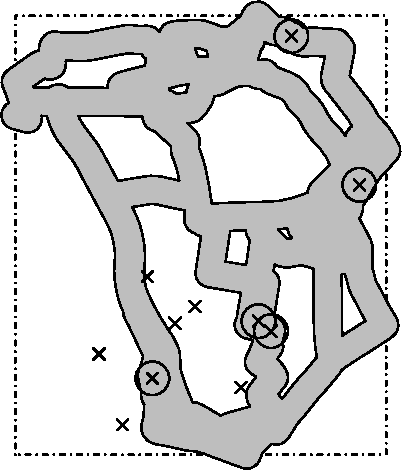
\includegraphics[width=0.5\linewidth]{fats-1}

}

\caption[Road traffic fatalities in the study area downloaded with with stplanr (crosses)]{Road traffic fatalities in the study area downloaded with with stplanr (crosses). Deaths that happened within 100 m of the route network are represented by circles.}\label{fig:fats}
\end{figure}
\end{Schunk}

\subsubsection{Reading census data} \label{reading-census-data}

National censuses are one common source of transport data, which frequently include questions on where people live and work.
This is often accompanied by a question on what mode was taken.
These data are generally provided in standard tables that can be downloaded for free.
For the Australian census, both these standard tables are available as well as custom tables that can be produced using a service named TableBuilder.
TableBuilder generates Excel or CSV files that contain additional lines that make reading these data into R difficult.
\textbf{stplanr} provides the \texttt{read\_table\_builder} function to read in these files.

Using the example \texttt{SA1Population.xlsx} file included with \textbf{stplanr} that contains the population by SA1 zone (a statistical area used for the Australian census), we can use the \texttt{read\_table\_builder} function to read and format the table for use in R.
The function automatically removes the additional lines and sets the column headers and data types as appropriate.
The result is a data.frame that can be used with GIS boundary files and other datasets produced for SA1 zones.

\begin{Schunk}
\begin{Sinput}
data_dir <- system.file("extdata", package = "stplanr")
t2 <- read_table_builder(file.path(data_dir, 'SA1Population.xlsx'),
                         filetype = 'xlsx', sheet = 1, removeTotal = TRUE)
\end{Sinput}
\end{Schunk}

\subsubsection{Bicycle share data} \label{bicycle-share-data}
\textbf{stplanr} can also be used in conjunction with complementary R packages for downloading data from Open Street Maps (OSM) using \CRANpkg{osmdata} and bicycle share data using the \CRANpkg{bikedata} package.

The bicycle share data that can be accessed using the \CRANpkg{bikedata} package is particularly well suited for integration with stplanr as it produces origin-destination (OD) flows from bicycle sharing systems.
This data can be used together with the \texttt{sum\_network\_links} function to generate the likely paths and how these overlap.
This can be used to generate heatmaps of a road network showing modelled common routes such as in Figure
\ref{fig:nyc-bicycle-data}.\footnote{The
figure is based on the shortest path, although other criteria could be used by setting weights in the network accordingly --- see \href{https://github.com/ropensci/stplanr/issues/194}{\#194} in the package's issue tracker for
details.}

\begin{figure}

{\centering 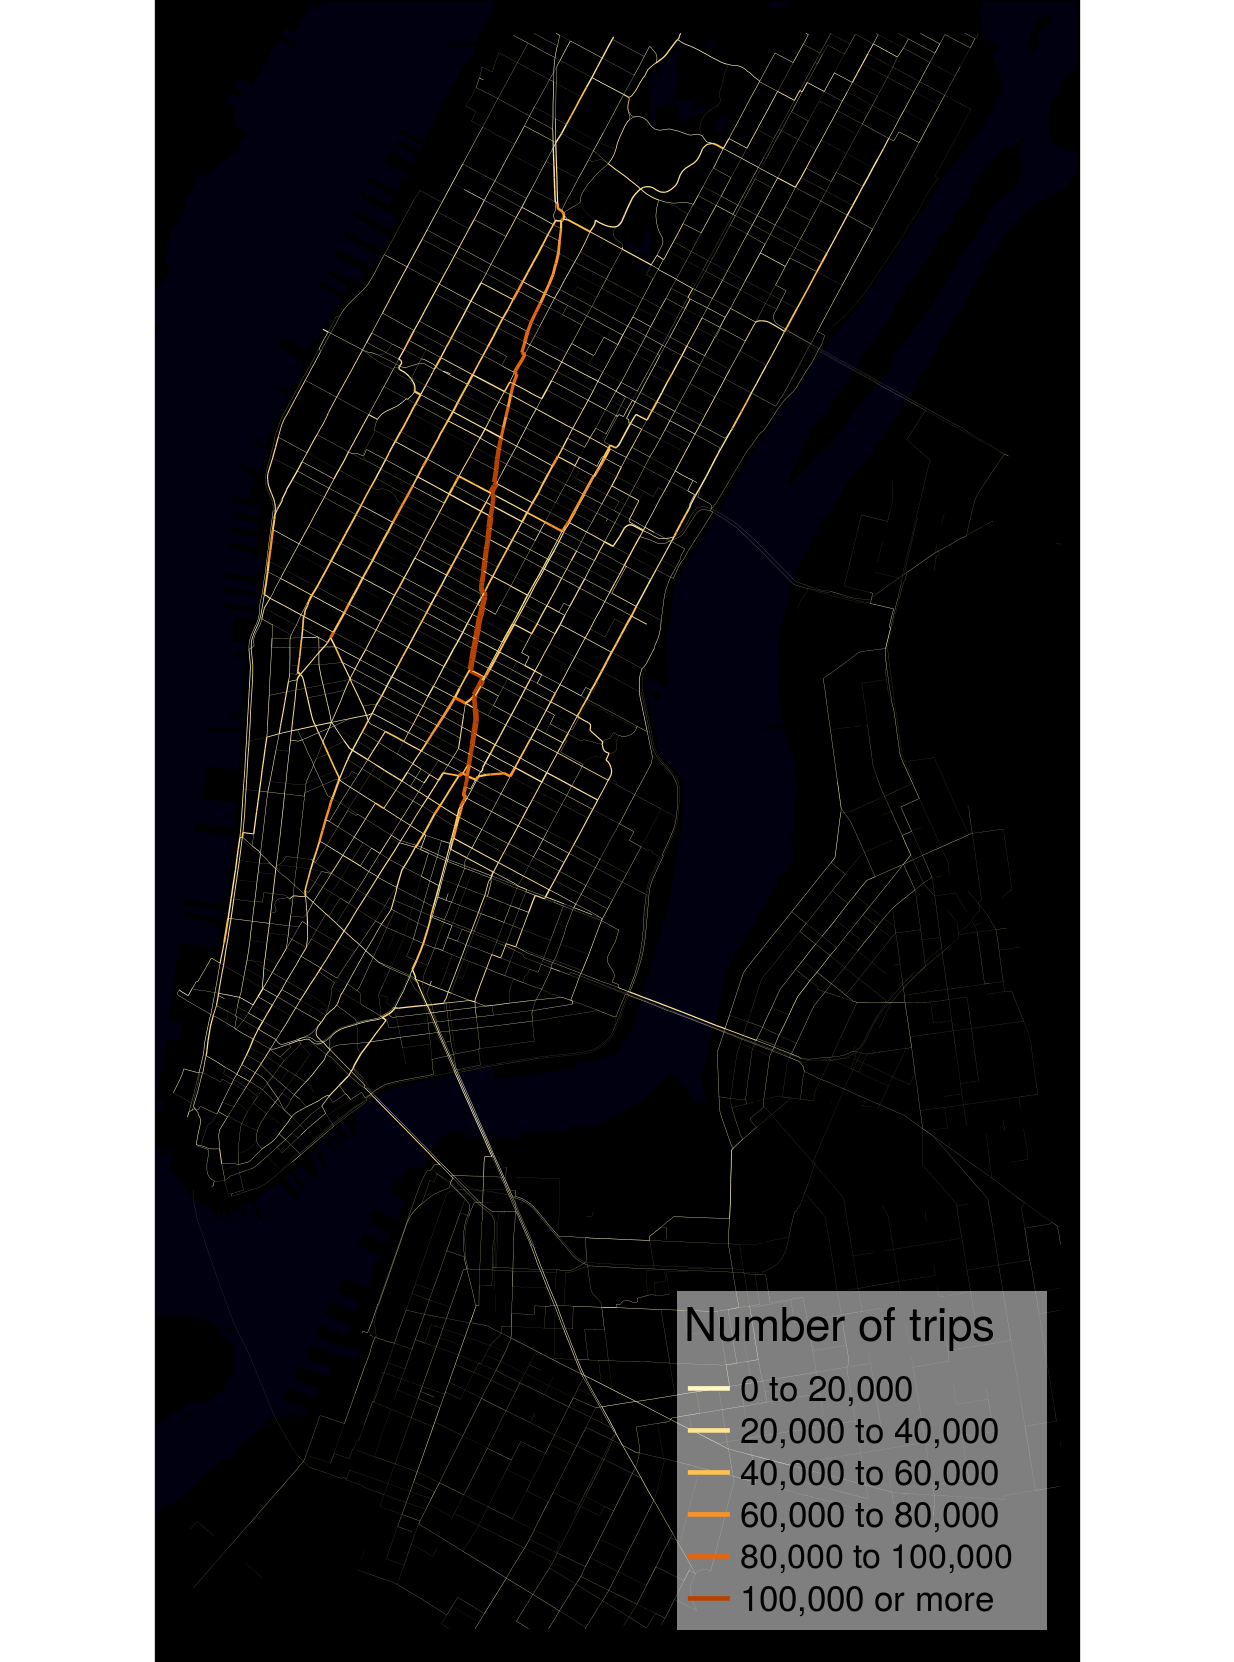
\includegraphics[width=0.55\linewidth]{nyc-bicycle-data}

}

\caption{Modelled common routes for bicycle share trips in New York City.}\label{fig:nyc-bicycle-data}
\end{figure}

\subsection{Creating geographic desire
lines}\label{creating-geographic-desire-lines}

% Clarify that this is an OD matrix in transport lingo
Origin-destination (`OD') data, which represent the number of people travelling between
geographical zones, is a key input for transport planning \citep{calabrese_estimating_2011}.
OD data usually represent an aggregate data source, and are therefore able to represent the
travel patterns of an entire country in a file of manageable size
(see \href{http://wicid.ukdataservice.ac.uk/}{wicid.ukdataservice.ac.uk/} for example).
They can be stored as a (sparse) matrix or (more commonly) a long table of OD pairs.
The long form is illustrated in the code chunk below which shows a sample of
the \texttt{flow} object.
\texttt{flow} is a \texttt{data.frame} representing the number
of home-work commutes by mode between residential
areas in the UK, provided provided in \CRANpkg{stplanr}
for teaching and demonstration purposes
(see \texttt{?flow} to see how this dataset was created):

\begin{Schunk}
\begin{Sinput}
data("flow", package = "stplanr")
head(flow[c(1:3, 12)])
\end{Sinput}
\begin{Soutput}
#>        Area.of.residence Area.of.workplace All Bicycle
#> 920573         E02002361         E02002361 109       2
#> 920575         E02002361         E02002363  38       0
#> 920578         E02002361         E02002367  10       0
#> 920582         E02002361         E02002371  44       3
#> 920587         E02002361         E02002377  34       0
#> 920591         E02002361         E02002382   7       0
\end{Soutput}
\end{Schunk}

Although the flow data displayed above describes movement over
geographical space, it contains no explicitly geographical information.
Instead, the coordinates of the origins and destinations are linked to a
separate geographical dataset (represented by the \texttt{cents} dataset),
as illustrated below:\footnote{Such geographic datasets are best represented as in a spatial class system, explaining
\textbf{stplanr}'s close integration with R's spatial packages.}


\begin{Schunk}
\begin{Sinput}
data("cents", package = "stplanr")
as.data.frame(cents[1:3, -c(3,4)])
\end{Sinput}
\begin{Soutput}
#>       geo_code  MSOA11NM coords.x1 coords.x2
#> 1708 E02002384 Leeds 055 -1.546463  53.80952
#> 1712 E02002382 Leeds 053 -1.511861  53.81161
#> 1805 E02002393 Leeds 064 -1.524205  53.80410
\end{Soutput}
\end{Schunk}

A common task is linking an OD dataset (e.g. \texttt{flow}) to a geographic dataset
representing zone centroids (e.g. \texttt{cents}).
We use \texttt{od2line} to combine them, as illustrated in the code chunk below,
which creates an object named \texttt{l} that will be visualised
in the next section:

\begin{Schunk}
\begin{Sinput}
l <- od2line(flow = flow, zones = cents)
\end{Sinput}
\end{Schunk}

\begin{figure}
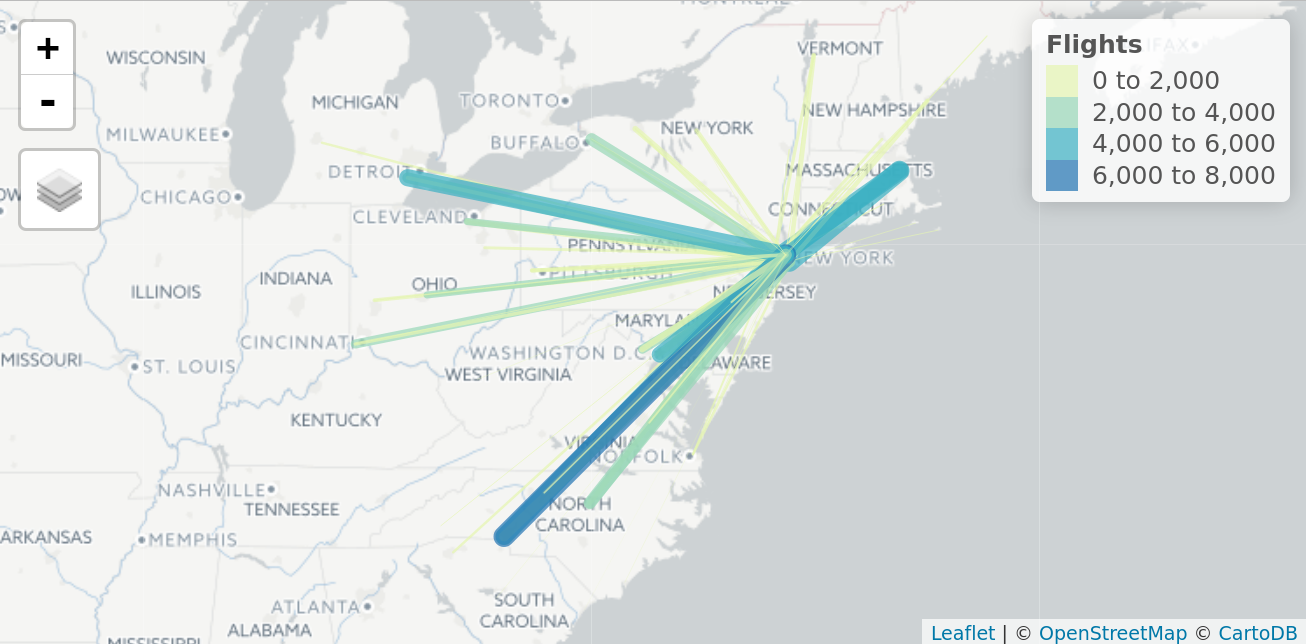
\includegraphics[width=\textwidth]{flights} \caption[Flights from New York]{Flights from New York to airports within 1000 km. Data from the \CRANpkg{nycflights} package converted to geographic desire lines with the \texttt{od2line} function.}\label{fig:flights}
\end{figure}

The resulting \texttt{l} object data is now in a spatial data class, enabling geographic analysis and
visualisation, as illustrated in Figure \ref{fig:lines_routes}.
A larger example of this desire line creation method is illustrated in \ref{fig:flights}, which also makes use of the function \texttt{buff\_geo}, is provided below based on a large dataset of flights from New York in 2013 from the \CRANpkg{nycflights13} package:

\begin{Schunk}
\begin{Sinput}
library(nycflights13)
data("airports")
crs <- CRS("+init=epsg:4326")
coords <- cbind(airports$lon, airports$lat)
airports_sp <- SpatialPointsDataFrame(coords, airports, proj4string = crs)
ny_buff <- buff_geo(shp = airports_sp[airports_sp$faa == "NYC",], width = 1e6)
airports_near <- airports_sp[ny_buff,]
flights_near <- flights[flights$dest %in% airports_near$faa,]
flights_agg <- group_by(flights_near, origin, dest) %>%
  summarise(Flights = n())
flights_sp = od2line(flow = flights_agg, zones = airports_near)
plot(flights_sp)
\end{Sinput}
\end{Schunk}

\subsection{Allocating flows to the transport
network}\label{allocating-flows-to-the-transport-network}

A common problem faced by transport researchers is network allocation:
converting the `as the crow flies' lines illustrated in the figure above
into routes. These are the complex, winding paths that people and
animals make to avoid obstacles such as buildings and to make the
journey faster and more efficient (e.g.~by following the route network).

This is difficult (and was until recently near impossible using free
software) because of the size and complexity of transport networks, the
complexity of realistic routing algorithms and need for
context-specificity in the routing engine. Inexperienced cyclists, for
example, would take a very different route than a heavy goods vehicle.
\textbf{stplanr} tackles this issue in two ways: by providing routing
functionality that can work on locally stored data and by using third party APIs.
Each approach has advantages: local routing functionality is fast and free,
whereas online routing services can be more sophisticated (e.g. taking
into account local traffic conditions) and work anywhere in the world
without needing to download unwieldy datasets and new software libraries such
as OSRM.
A disadvantage of relying on online services is that they may break or change
without warning in the future.

Route allocation is undertaken by \code{route\_} functions such as
\code{route\_cyclestreets} and \linebreak \code{route\_graphhopper}.
These allocate a single OD pair (represented by \texttt{from} and \texttt{to}
arguments as coordinates,
spatial point objects or text strings to be
`geo-coded') to the transport network.
This is illustrated
below with \texttt{route\_cyclestreet}, which uses the
\href{http://www.cyclestreets.net/api/}{CycleStreets.net API}, a routing
service ``by cyclists for cyclists'' which provides
`fastest', `quietest' and `balanced' routes:\footnote{An
API key
  is needed for this function to work. This can be requested (or
  purchased for large scale routing) from
  \href{https://www.cyclestreets.net/api/apply/}{cyclestreets.net/api/apply}.
  See \texttt{?route\_cyclestreet} for details. Thanks to Martin
  Lucas-Smith and Simon Nuttall for making this possible.}

\begin{Schunk}
\begin{Sinput}
route_bl <- route_cyclestreet(from = "Bradford, Yorkshire", to = "Leeds, Yorkshire")
route_c1_c2 <- route_cyclestreet(cents[1,], cents[2,])
\end{Sinput}
\end{Schunk}

The raw output from routing APIs is usually provided as a JSON or
GeoJSON text string. By default, \texttt{route\_cyclestreet} saves a
number of key variables (including length, time, hilliness and busyness
variables generated by CycleStreets.net) from the attribute data
provided by the API. If the user wants to save the raw output, the
\texttt{save\_raw} argument can be used:

\begin{Schunk}
\begin{Sinput}
route_bl_raw <- route_cyclestreet(from = "Bradford", to = "Leeds", save_raw = TRUE)
\end{Sinput}
\end{Schunk}

Additional arguments taken by the \texttt{route\_} functions depend on
the routing function in question. By changing the \texttt{plan} argument
of \texttt{route\_cyclestreet} to \texttt{fastest}, \texttt{quietest} or
\texttt{balanced}, for example, routes favouring speed, quietness or a
balance between speed and quietness will be saved, respectively.

To automate the creation of route-allocated lines over many desire
lines, the \texttt{line2route} function loops over each line, wrapping
any \texttt{route\_} function as an input. The output is a
\texttt{SpatialLinesDataFrame} with the same number of dimensions as the
input dataset (see the right panel in Figure \ref{fig:lines_routes}).

\begin{verbatim}
routes_fast <- line2route(l = l, route_fun = route_cyclestreet)
\end{verbatim}

The result of this `batch routing' exercise is illustrated in Figure
\ref{fig:lines_routes}. The red lines in the left hand panel are very
different from the hypothetical straight `desire lines', highlighting the importance of this route-allocation
functionality (see \texttt{vignette("introducing-stplanr")} and \href{http://kateto.net/network-visualization}{kateto.net} for more sophisticated visualisation methods).

\begin{Schunk}
\begin{Sinput}
plot(route_network, lwd=0)
plot(l, lwd = l$All / 10, add = TRUE)
lines(routes_fast, col = "red")
routes_fast$All <- l$All
rnet <- overline(routes_fast, "All", fun = sum)
rnet$flow <- rnet$All / mean(rnet$All) * 3
plot(rnet, lwd = rnet$flow / mean(rnet$flow))
\end{Sinput}
\begin{figure}
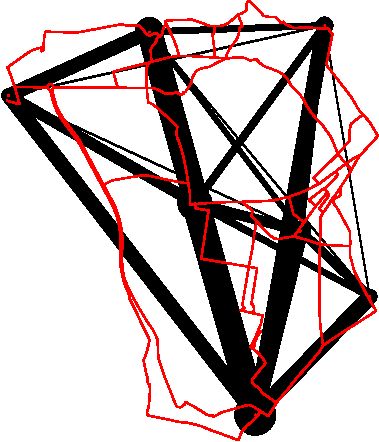
\includegraphics[width=0.5\linewidth]{lines_routes-1} 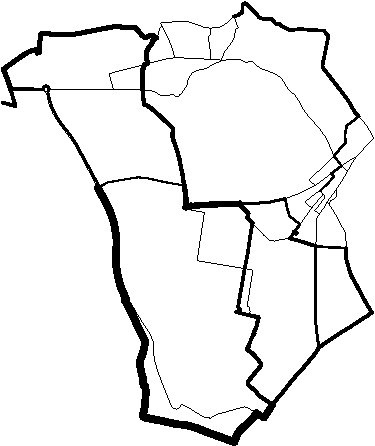
\includegraphics[width=0.5\linewidth]{lines_routes-2} \caption[Visualisation of travel desire lines, with width proportional to number of trips between origin and destination (black) and routes allocated to network  (red) in the left-hand panel]{Visualisation of travel desire lines, with width proportional to number of trips between origin and destination (black) and routes allocated to network  (red) in the left-hand panel. The right hand panel shows the route network dataset generated by overline().}\label{fig:lines_routes}
\end{figure}
\end{Schunk}

To estimate the amount of capacity needed at each segment on the
transport network, the \texttt{overline} function demonstrated above, is
used to divide line geometries into unique segments and aggregate the
overlapping values. The results, illustrated in the right-hand panel of
Figure \ref{fig:lines_routes}, could be used to informt the decision making process at the route network level, such as where to create new bus routes cycle paths.

Limitations with the \texttt{route\_cyclestreet} routing API include its
specificity, to one mode (cycling) and a single region (the UK and part
of Europe). To overcome these limitations, additional routing APIs were
added with the functions \texttt{route\_graphhopper},
\texttt{route\_transportapi\_public} and \texttt{viaroute}. These
interface to Graphhopper, TransportAPI and the Open Source Routing
Machine (OSRM) routing services, respectively.
Advanced users can set-up local routing services (as demonstrated in a guide by
\href{https://www.digitalocean.com/community/tutorials/how-to-set-up-an-osrm-server-on-ubuntu-14-04}{DigitalOcean}), reducing the disadvantages of using online routing services:
they rely on on potentially slow internet connections, changeable APIs,
and variable/high prices.

A short example of finding the route by car and bike between New York
and Oaxaca demonstrates how \texttt{route\_graphhopper} can collect
geographical and other data on routes by various modes, anywhere in the
world. The output, shown in Table \ref{tab:xtnyoa}, shows that the
function also saves time, distance and (for bike trips) vertical
distance climbed for the trips.

\begin{Schunk}
\begin{Sinput}
ny2oaxaca1 <- route_graphhopper("New York", "Oaxaca", vehicle = "bike")
ny2oaxaca2 <- route_graphhopper("New York", "Oaxaca", vehicle = "car")
rbind(ny2oaxaca1@data, ny2oaxaca2@data)
\end{Sinput}
\end{Schunk}

\begin{longtable}[]{@{}lrrr@{}}
\toprule
mode & time & dist & change\_elev\tabularnewline
\midrule
\endhead
Bike & 17522.73 & 4885663 & 87388.13\tabularnewline
Car  &   2759.89 & 4754772 & NA\tabularnewline
\bottomrule
\caption[Results obtained from the Graphhopper API]{Results obtained from the Graphhopper API using the \code{route\_graphhopper} function to estimate the time taken and route distance to travel between New York and Oaxaca by cycling and driving.}
\label{tab:xtnyoa}
\end{longtable}

\subsection{Modelling travel catchment
areas}\label{modelling-travel-catchment-areas}

Accessibility to transport services, meaning ease of access rather than
it simply being possible to get somewhere, is an important topic
when considering public transport or active travel because of the
steep reduction in use with distance to services (or
infrastructure). As a result, the planning for transport
services and infrastructure frequently focuses on several measures of
accessibility including distance, but also travel times and frequencies
and weighted by population. The functions in \textbf{stplanr} are
intended to provide a method of estimating these accessibility measures
as well as calculating the population that can access specific services
(i.e., estimating the catchment area).

Catchment areas in particular are a widely used measure of accessibility
that attempts to both quantify the likely target group for a particular
service, and visualise the geographic area that is covered by the
service. For instance, passengers are often said to be willing to walk
up to 400 metres to a bus stop, or 800 metres to a railway station
\citep{el-geneidy_new_2014}. Although these distances may appear
relatively arbitrary and have been found to underestimate the true
catchment area of bus stops and railway stations
\citep{el-geneidy_new_2014,daniels_explaining_2013} they nonetheless
represent a good, albeit somewhat conservative, starting point from
which catchment areas can be determined.

In many cases, catchment areas are calculated on the basis of
straight-line (or ``as the crow flies'') distances. This is a
simplistic, but relatively appealing approach because it requires little
additional data and is straight-forward to understand. \textbf{stplanr}
provides functionality that calculates catchment areas using
straight-line distances with the \texttt{calc\_catchment} function. This
function takes a \texttt{SpatialPolygonsDataFrame} that contains the
population (or other) data, typically from a census, and a
\texttt{Spatial*} layer that contains the geometry of the transport
facility. These two layers are overlayed to calculate statistics for the
desired catchments including proportioning polygons to account for the
proportion located within the catchment area.

\newpage

To illustrate how catchment areas can be calculated, \textbf{stplanr}
contains some sample datasets stored in ESRI Shapefile format (a
commonly used format for distributing GIS layers) that can together be
used to calculate sample catchment areas. One of these datasets
(\texttt{smallsa1}) contains population data for Statistical Area 1
(SA1) zones in Sydney, Australia. The second contains hypothetical
cycleways aligned to streets in Sydney. The code below unzips the
datasets and reads in the shapefiles using the \texttt{readOGR} function
of \CRANpkg{rgdal}.

\begin{Schunk}
\begin{Sinput}
data_dir <- system.file("extdata", package = "stplanr")
unzip(file.path(data_dir, 'smallsa1.zip'))
unzip(file.path(data_dir, 'testcycleway.zip'))
sa1income <- rgdal::readOGR(".", "smallsa1")
testcycleway <- rgdal::readOGR(".", "testcycleway")
# Remove unzipped files
file.remove(list.files(pattern = "^(smallsa1|testcycleway).*"))
\end{Sinput}
\end{Schunk}

Calculating the catchment area is straightforward and in addition to
specifying the required datasets, only a vector containing column names
to calculate statistics and a distance is required. Since proportioning
the areas assumes projected data, unprojected data are automatically
projected to either a common projection (if one is already projected) or
a specified projection. It should be emphasised that the choice of
projection is important and has an effect on the results meaning setting
a local projection is recommended to achieve the most accurate results.

\begin{Schunk}
\begin{Sinput}
catch800m <- calc_catchment(
  polygonlayer = sa1income,
  targetlayer = testcycleway,
  calccols = c('Total'),
  distance = 800,
  projection = 'austalbers',
  dissolve = TRUE
)
\end{Sinput}
\end{Schunk}

By looking at the data.frame associated with the
SpatialPolygonsDataFrame that is returned from the
\texttt{calc\_catchment} function, the total population within the
catchment area can be seen to be 39418 people. The catchment area
is plotted using the
\texttt{plot} function as illustrated in
the code below (see
Figure \ref{fig:catchmentplot}).

\begin{Schunk}
\begin{Sinput}
plot(sa1income, col = "light grey")
plot(catch800m, col = rgb(1, 0, 0, 0.5), add = TRUE)
plot(testcycleway, col = "green", add = TRUE)
\end{Sinput}
\begin{figure}
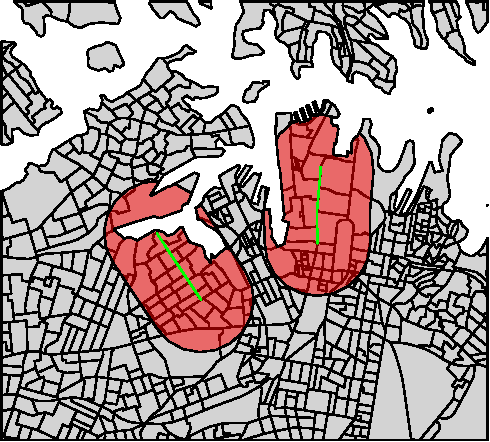
\includegraphics[center]{catchmentplot-1} \caption[An 800 metre catchment area (red) associated with a cycle path (green) using straight-line distance in Sydney]{An 800 metre catchment area (red) associated with a cycle path (green) using straight-line distance in Sydney.}\label{fig:catchmentplot}
\end{figure}
\end{Schunk}

This simplistic catchment area is useful when the straight-line distance
is a reasonable approximation of the route taken to walk (or cycle) to a
transport facility. However, this is often not the case. The catchment
area in Figure \ref{fig:catchmentplot} initially appears reasonable but
the red-shaded catchment area includes an area that requires travelling
around a bay to access from the (green-coloured) cycleway:
users may have \emph{access} but that does not mean it's \emph{accessible}. To allow for
more realistic catchment areas for most situations, \textbf{stplanr}
provides the \texttt{calc\_network\_catchment} function that uses the
same principle as \texttt{calc\_catchment} but also takes into account
the transport network.

To use \texttt{calc\_network\_catchment}, a transport network needs to
be prepared that can be used in conjunction with the previous datasets.
Preparation of the dataset involves using the
\texttt{SpatialLinesNetwork} function to create a network from a
\texttt{SpatialLinesDataFrame}. This function combines a
\texttt{SpatialLinesDataFrame} with a graph network (using the
\CRANpkg{igraph} package) to provide basic routing functionality. The
network is used to calculate the shortest actual paths within the
specific catchment distance. This process involves the following code:

\begin{Schunk}
\begin{Sinput}
unzip(file.path(data_dir, 'sydroads.zip'))
sydroads <- rgdal::readOGR(".", "roads")
file.remove(list.files(pattern = "^(roads).*"))
sydnetwork <- SpatialLinesNetwork(sydroads)
\end{Sinput}
\end{Schunk}

The network catchment is then calculated using a similar method as with
\texttt{calc\_catchment} but with a few minor changes. Specifically
these are including the \texttt{SpatialLinesNetwork}, and using the
\texttt{maximpedance} parameter to define the distance, with distance
being the additional distance from the network. In contrast to the
distance parameter that is based on the straight-line distance in both
the \texttt{calc\_catchment} and \texttt{calc\_network\_catchment}
functions, the \texttt{maximpedance} parameter is the maximum value in
the units of the network's weight attribute. In practice this is
generally distance in metres but can also be travel times, risk or other
measures.

\begin{Schunk}
\begin{Sinput}
netcatch800m <- calc_network_catchment(
  sln = sydnetwork,
  polygonlayer = sa1income,
  targetlayer = testcycleway,
  calccols = c('Total'),
  maximpedance = 800,
  distance = 100,
  projection = 'austalbers'
)
\end{Sinput}
\end{Schunk}

Once calculated, the network catchment area can be used just as the
straight-line network catchment. This includes extracting the catchment
population of 23457 and plotting the original catchment area together
with the original area with the results shown in Figure
\ref{fig:netcatchplot}:

\begin{Schunk}
\begin{Sinput}
plot(sa1income, col = "light grey")
plot(catch800m, col = rgb(1, 0, 0, 0.5), add = TRUE)
plot(netcatch800m, col = rgb(0, 0, 1, 0.5), add = TRUE)
plot(testcycleway, col = "green", add = TRUE)
\end{Sinput}
\begin{figure}
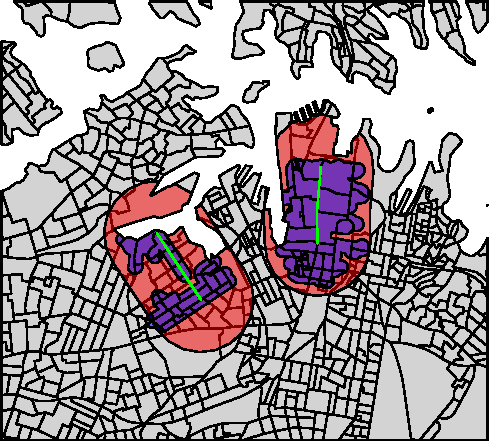
\includegraphics[center]{netcatchplot-1} \caption[A 800 metre network catchment are (blue) compared with a catchment area based on Euclidean distance (red) associated with a cycle path (green)]{A 800 metre network catchment are (blue) compared with a catchment area based on Euclidean distance (red) associated with a cycle path (green).}\label{fig:netcatchplot}
\end{figure}
\end{Schunk}

\texttt{calc\_catchment} and \texttt{calc\_network\_catchment} provide complementary functions that allow for the computation of catchment areas.
Although for many transport applications it would be better to use the \texttt{calc\_network\_catchment} function that uses the true network distances, it may still be useful to use the straight-line version in some cases.
These include calculating the population that may be affected by noise levels from transport infrastructure (such as a motorway) where the effects of noise are not limited by the network.
In situations where network data is not available it would be possible to use the \texttt{calc\_catchment} function together with a fixed assumption about what straight-line distance corresponds to the desired network distance (i.e., 1km network = 700m straight-line).
It may also be appropriate to use the straight-line distance when the network is not a reasonable constraint.
This may be because the infrastructure of interest is accessed primarily by walking or cycling in an area where these are not limited to the road network (such as parks or shopping areas with passthroughs or overpasses available to pedestrians).

\section{Modelling and visualisation}\label{modelling-and-visualisation}

\subsection{Analysing mode use}\label{modelling-mode-choice}

Route-allocated lines allow estimation of \emph{route distance} and therefore
\emph{circuity ($Q$)} (route distance divided by Euclidean distance)
\citep{levinson_minimum_2009}:

\[
 Q = \frac{d_{Rf}}{d_E}
\]

where (\(d_E\)) and (\(d_{Rf}\)) represent
Euclidean and fastest route distance respectively.

These
variables can help model the rate of flow between origins and
destination, as illustrated in the left-hand panel of Figure
\ref{fig:euclidfastest}. The code below demonstrates how objects
generated by \textbf{stplanr} can be used to undertake such analysis,
with the \texttt{line\_length} function used to find the distance, in
meters, of lat/lon data.

\begin{verbatim}
l$d_euclidean <- line_length(l)
l$d_rf <- routes_fast@data$length
plot(l$d_euclidean, l$d_rf,
  xlab = "Euclidean distance", ylab = "Route distance")
abline(a = 0, b = 1)
abline(a = 0, b = 1.2, col = "green")
abline(a = 0, b = 1.5, col = "red")
\end{verbatim}

The left hand panel of Figure \ref{fig:euclidfastest} shows the expected
strong correlation between Euclidean (\(d_E\)) and fastest route
(\(d_{Rf}\)) distance. However, some OD pairs have a proportionally
higher route distance than others, as illustrated by distance from the
black line in the above plot.

An extension to the concept of circuity is the `quietness diversion
factor' (\(QDF\)) of a desire line \citep{lovelace_propensity_2017}, the
ratio of the route distance of a quiet route option (\(d_{Rq}\)) to that
of the fastest:

\[
 QDF = \frac{d_{Rq}}{d_{Rf}}
\]

Thanks to the `quietest' route option provided by
\texttt{route\_cyclestreet}, we can estimate average values for both
metrics as follows:

\begin{Schunk}
\begin{Sinput}
routes_slow <- line2route(l, route_cyclestreet, plan = "quietest")
\end{Sinput}
\end{Schunk}

\begin{Schunk}
\begin{Sinput}
l$d_rq <- routes_slow$length # quietest route distance
Q <- mean(l$d_rf / l$d_euclidean, na.rm = TRUE)
QDF <- mean(l$d_rq / l$d_rf, na.rm = TRUE)
Q
\end{Sinput}
\begin{Soutput}
#> [1] 1.298767
\end{Soutput}
\begin{Sinput}
QDF
\end{Sinput}
\begin{Soutput}
#> [1] 1.034721
\end{Soutput}
\end{Schunk}

The results show that cycle paths are not particularly direct in the
study region by international standards \citep{crow_design_2007}. This
is hardly surprisingly given the small size of the sample and the short
distances covered: \(Q\) tends to decrease at a decaying rate with
distance, meaning longer paths tend to be more direct.
What is surprising is that the quietness diversion factor
\(QDF\) is close to unity, which
could imply that the quiet routes are constructed along direct, and
therefore sensible routes.
When time is
explored, we find that the `quietness diversion factor with respect to
time' (\(QDF_t\)) is slightly larger,
although larger datasets would be needed for any inferences to be made:

\begin{Schunk}
\begin{Sinput}
(QDFt <- mean(routes_slow$time / routes_fast$time, na.rm = TRUE))
\end{Sinput}
\begin{Soutput}
#> [1] 1.052855
\end{Soutput}
\end{Schunk}

\subsection{Analysing and estimating trip flows}\label{models-of-travel-behaviour}

The second step in the four-stage transport model (after trip generation) is trip distribution.
This involves identifying destinations for trips generated in each zone (creating OD data), which can be done with a gravity model, logit model, or other technique under the broad banner of `spatial interaction model' (SIM).
\textbf{stplanr} is not intended primarily as a SIM package, but could be extended in this direction, as illustrated by \texttt{od\_radiation} function, which implements a SIM proposed by \citet{simini_universal_2012}.
Further development in this direction (or integration with a package dedicated to SIMs) would complement \textbf{stplanr}'s focus on geographic functions.

At present there are no functions for modelling distance decay, but this
is something we would like to add in future versions of
\textbf{stplanr}.
Although it is only one of several methods used for modelling trip distribution as part of four-step models,
distance decay is an especially important concept for
sustainable transport planning due to physical limitations on the
ability of people to walk and cycle large distances
\citep{iacono_measuring_2010}.
It can also be used to model relationships between locations in situations that are sensitive to distance (cycling facilities for instance) in addition to its use in four-step models.

We can explore the relationship between distance and the proportion of
trips made by walking, using the same object \texttt{l} generated by
\textbf{stplanr}.

\begin{Schunk}
\begin{Sinput}
l$pwalk <- l$On.foot / l$All
plot(l$d_euclidean, l$pwalk, cex = l$All / 50,
  xlab = "Euclidean distance (m)", ylab = "Proportion of trips by foot")
\end{Sinput}
\end{Schunk}

\begin{Schunk}
\begin{figure}
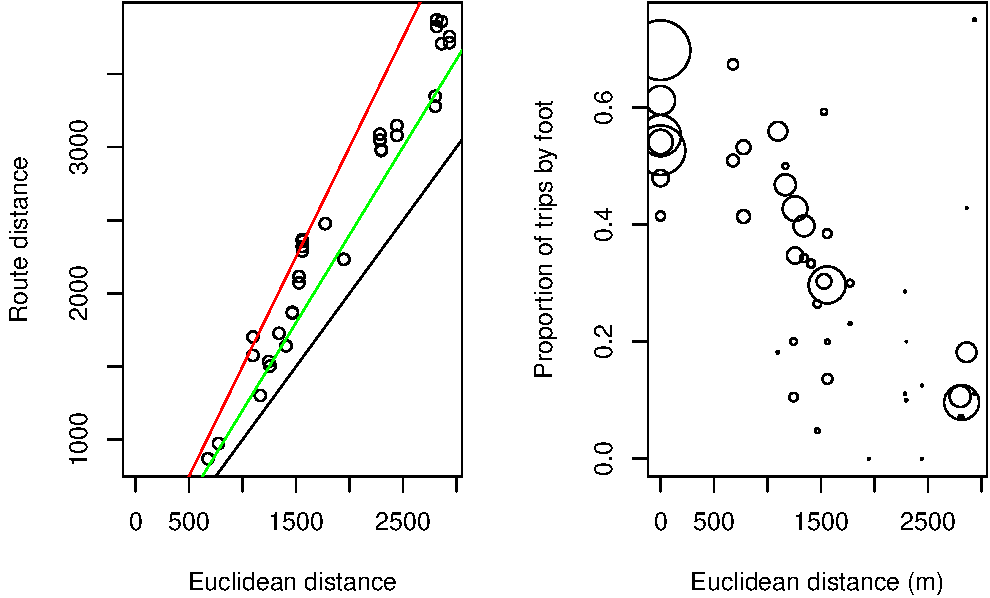
\includegraphics[width=1\linewidth]{euclidfastest-1} \caption[Euclidean and fastest route distance of trips in the study area (left) and Euclidean distance vs the proportion of trips made by walking (right)]{Euclidean and fastest route distance of trips in the study area (left) and Euclidean distance vs the proportion of trips made by walking (right).}\label{fig:euclidfastest}
\end{figure}
\end{Schunk}

Based on the right-hand panel in Figure \ref{fig:euclidfastest}, there
is a clear negative relationship between distance of trips and the
proportion of those trips made by walking. This is unsurprising: beyond
a certain distance (around 1.5km according the the data presented in the
figure above) walking is usually seen as too slow and other modes are
considered.
This `distance decay' is non-linear and can be approximated by a range of functional forms \citep{martinez_new_2013}.
From the range of
options we test below just two forms. We will compare the ability of
linear and log-square-root functions to fit the data contained in
\texttt{l} for walking.

\begin{Schunk}
\begin{Sinput}
lm1 <- lm(pwalk ~ d_euclidean, data = l@data, weights = All)
lm2 <- lm(pwalk ~ d_rf, data = l@data, weights = All)
lm3 <- glm(pwalk ~ d_rf + I(d_rf^0.5),
           data = l@data, weights = All, family = quasipoisson(link = "log"))
\end{Sinput}
\end{Schunk}

The results of these regression models can be seen using
\texttt{summary()}. Surprisingly, Euclidean distance was a better
predictor of walking than route distance, but no strong conclusions can
be drawn from this finding, with such a small sample of desire lines (n
= 42). The results are purely illustrative, of the
possibilities created by using \textbf{stplanr} in conjuction with R's
modelling capabilities (see Figure \vref{fig:euclidwalking2}).

\begin{Schunk}
\begin{Sinput}
plot(l$d_euclidean, l$pwalk, cex = l$All / 50,
  xlab = "Euclidean distance (m)", ylab = "Proportion of trips by foot")
l2 <- data.frame(d_euclidean = 1:5000, d_rf = 1:5000)
lm1p <- predict(lm1, l2)
lm2p <- predict(lm2, l2)
lm3p <- predict(lm3, l2)
lines(l2$d_euclidean, lm1p)
lines(l2$d_euclidean, exp(lm2p), col = "green")
lines(l2$d_euclidean, exp(lm3p), col = "red")
\end{Sinput}
\begin{figure}

{\centering 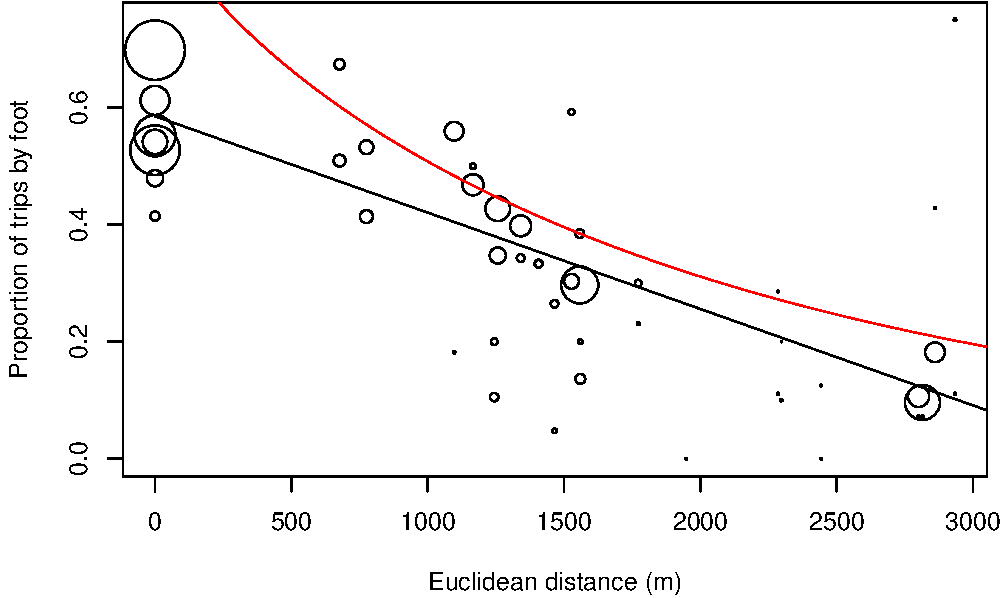
\includegraphics[width=0.75\linewidth]{euclidwalking2-1}

}

\caption[Relationship between euclidean distance and walking]{Relationship between euclidean distance and walking}\label{fig:euclidwalking2}
\end{figure}
\end{Schunk}

\subsection{Visualisation}\label{visualisation}

Visualisation is an important aspect of any transport study, as it
enables researchers to communicate their findings to other researchers,
policy-makers and, ultimately, the public. It may therefore come as a
surprise that \textbf{stplanr} contains no functions for visualisation.
Instead, users are encouraged to make use of existing spatial
visualisation tools in R, such as \textbf{tmap}, \textbf{leaflet} and
\textbf{ggmap} \citep{cheshire_spatial_2015,kahle_ggmap:_2013}.

Furthermore, with the development of online application frameworks such
as \textbf{shiny}, it is now easier than ever to make the results of
transport analysis and modelling projects available to the public.
There is great potential to expand on
the principle of publicly accessible transport planning tools via `web
apps', perhaps through new R packages dedicated to visualising
and communicating transport data.

\section{Future directions of travel}\label{future-directions-of-travel}

This paper demonstrates that transort planning can be done with open source, scriptable software.
We set out reasons for using R for transport planning and demonstrated the possibilities in the area of spatial data analysis for active travel planning with reproducible examples from \CRANpkg{stplanr}.
This is, to our knowledge, is the first R package aimed specifically to help practitioners and researchers design more sustainable transport systems.
However, much more is possible in this direction.
% Indeed, transport planning is a large and highly diverse area.
% Add this as a footnote?
% Transport planning has links to areas of knowledge which are already well-served by packages have yet to receive much (if any) attention from the transport community statistical networks, activity space analysis and the development of interactive online visualisations to encourage public engagement in the process.

The focus of \CRANpkg{stplanr} on geographic transport data was originally driven by the author's research interests.
However, we believe there are good reasons to continue this focus.
Proprietary software such as \href{https://www.inrosoftware.com/en/products/emme/}{INRO}, \href{http://vision-traffic.ptvgroup.com/en-us/products/ptv-visum/}{PTV Visum} and  \href{http://www.caliper.com/tcovu.htm}{TransCAD} dominate geospatial methods in applied transport planning.
This differs from other fields that use geospatial methods such spatial epidemiology and ecology, where open source software dominate.
Furthermore, the successful `unix approach' to software development implies that each piece of software does a limited number of things well.
To avoid the pitfall of `feature creep' it makes sense to specialise.

The lack of existing packages that do the same job direct our attention towards \textbf{stplanr}'s basic functionality rather than more advanced and esoteric features.
A good example of this is the \code{SpatialLinesNetwork} class which could provide a basis for future developments including a \code{route\_sln} function to facilitate routing in R, without recourse to external services.
This direction of `incremental growth' could proceed by adding interfaces to more transport planning APIs, including \href{https://www.routino.org/uk/}{Routino} and \href{https://www.mapbox.com/directions/}{Directions} provided by mapping company Mapbox, mitigating the limitations of online API services.

Another example of the potential to develop basic functionality rather than new advanced features is the the possibility of creating an `\code{OD}' class to represent origin-destination data, which could ease the geographical analysis of OD data via generic methods.
Building on the example data presented in previous sections the idea is for a single \code{OD} object to be able represent \code{flowlines}, \code{routes\_fast} and \code{routes\_quiet}.
The recent development of the \CRANpkg{sf} (discussed below), with its support for multiple geometry columns, makes this option more feasible.

Another desirable direction of travel is towards better support for large datasets.
We have demonstrated \textbf{stplnr}'s capabilities on deliberately small datasets for ease of understanding.
However, the third criterion of transport planning software set-out in the introduction --- \emph{scalability} --- is vital to package's real world utility in the age of transport-related `Big Data' \citep{lovelace_big_2016}.
For this reason we have endeavoured to use efficient programming techniques package functions and use C++ (via \CRANpkg{Rcpp}) for computationally intensive operations on \code{SpatialLinesNetwork}.
\CRANpkg{stplanr} was first developed to generate data for the national
Propensity to Cycle Project, which involved generating geographic desire lines for over 700,000 routes \citep{lovelace_propensity_2017} (and in Phase 2, over 4 million).
This experience led to a number of optimisations in the code, including an implementation a faster implementation of the \code{od2line} function (\code{od2line2}) and a commit that led to a 10 fold speed-up in the \code{line2route} function (see commit \href{https://github.com/ropensci/stplanr/commit/c834abf7d0020c6fbb33845572d6be4801f31f47}{c834abf}).

However, there are still opportunities for improving performance, including:
integration with transport databases (e.g. via the \CRANpkg{bikedata} package);
support for batch routing APIs;
parallel implementations of time-consuming functions;
and the refactoring of slow functions (e.g. \code{overline}, which takes hours to run on large datasets).

% and free accessibility makes it well-suited
% to the needs of transport planners and researchers, especially those
% wanting to avoid the high costs of market-leading products. Rather than
% `reinvent the wheel' (e.g.~with a new class system), \textbf{stplanr}
% builds on existing packages and \CRANpkg{sp} classes to work with common
% transport data formats.

It is useful to see \textbf{stplanr}, and R for transport planning in
general, as an addition tool in the transport planner's cabinet. It can
be understood as one part of a wider movement that is making transport
planning a more open and democratic process. Other developments in this
movement include the increasing availability of open data
\citep{naumova_building_2016} and the rise of open source products for
transport modelling, such as
\href{http://www.dlr.de/ts/en/desktopdefault.aspx/tabid-9883/16931_read-41000/}{SUMO},
\href{http://www.matsim.org/}{MATSim} and
\href{https://its.mit.edu/software/mitsimlab}{MITSIMLAB}
\citep{saidallah_comparative_2016} and
\href{http://pgrouting.org/}{pgRouting}.
In this context, \textbf{stplanr}'s focus on
GIS operations represents a niche in the market, allowing it to
complement such software and help make better use of new open data
sources.

Furthermore \textbf{stplanr} could be used alongside other R packages that
would benefit from spatial transport data as input.
These include packages for activity space analysis (e.g. \CRANpkg{aspace}) and
service location planning (e.g. \CRANpkg{MCI}) \citep{RJ-2017-020}.


Because transport planning is an inherently spatial activity,
\textbf{stplanr} occupies an important niche in the transport planning
software landscape, with its focus on spatial transport data. There is
great potential for development of \textbf{stplanr} in many directions.
Desirable developments include the additional of functions for modelling
modal split and improving the computational efficiency of
existing functions to make the methods more scalable for large
databases. Our priority for \textbf{stplanr} however, is to keep the
focus on geographic functions for transport planning. There are many
opportunities in this direction, including:

\begin{itemize}
\tightlist
\item
  Functions to assess the environment surrounding routes, e.g.~via
  integration with the in-development \textbf{osmdata} package.
\item
  Functions to match different GIS routes, perhaps building on the
  Hausdorf distance algorithm implemented in the \CRANpkg{rgeos}
  function \texttt{gDistance}.
\item
  Additional functions for route-allocation of travel, e.g.~via an
  interface to the OpenTripPlanner API.
\item
  Functions for aggregating very large GPS trace datasets (e.g.~into
  raster cells) for anonymisation and analysis/visualisation purposes.
\item
  The creation of a class system for spatial transport datasets, such as
  to represent spatial route and a route networks (perhaps with classes
  named \code{"sr"} and \code{"srn"}). This is not a short-term priority
  and it would be beneficial to coincide such developments to a
  migration to \CRANpkg{sf} for spatial classes.
\end{itemize}

Such spatial data processing capabilities would increase the range of
transport planning tasks that \textbf{stplanr} can facilitate. For all
this planned development activity to be useful, it is vital that new
functionality is user friendly. R has a famously steep learning curve.
Implementing simple concepts such as consistent naming systems
\citep{baath_state_2012} and ensuring `type stability' can greatly
improve the usability of the package. For this reason, much future work
in \textbf{stplanr} will go into improving documentation and
user-friendliness.

We have set out clear motivations for
developing transport planning capabilities in R and believe that
\textbf{stplanr} provides major a step in that direction.
However, it is important to recognise that open source software is
a broad church with many alternative and potentially mutually beneficial
projects existing in parallel.
In the context of the increasing availability of open access data\footnote{Two
examples of this are the \CRANpkg{osmdata} CRAN package \citep{Padgham2017} and the Python package
\href{https://github.com/gboeing/osmnx}{OSMnx} \citep{boeing_osmnx:_2017}, for downloading and processing
open access datasets from OpenStreetMap.}
packages for analysing transport datasets such as \CRANpkg{stplanr} could help
ensure that the
evidence on which transport planning decisions are based is reproducible,
systematic, and therefore more democratically accountable.

\section{Acknowledgements}

We would like to thank a number of people and organisations who have supported the development of \CRANpkg{stplanr}:
the UK's Department for Transport (DfT) for funding the Propensity to Cycle Tool (see \href{http://www.pct.bike/}{www.pct.bike})
which instigated code which eventually became \textbf{stplanr};
Colin Gillespie, whose teaching helped turn the code into a package;
ROpenSci, for hosting the package (special thanks to Scott Chamberlin who reviewed the package);
to Ma{\"e}lle Salmon, Mark Padgham, Martin Lucas-Smith and Marcus Young for commenting on early drafts of this paper;
and to transport planning professionals Tom van Vuren (Mott MacDonald), John Parkin (University of the West of England), Helen Bowkett (Welsh Government) and Yaron Hollander, who provided input on the paper and ideas for future priorities.

\bibliography{references}

\address{%
Robin Lovelace\\
University of Leeds\\
34-40 University Road\\ LS2 9JT, UK\\
}
\href{mailto:r.lovelace@leeds.ac.uk}{\nolinkurl{r.lovelace@leeds.ac.uk}}

\address{%
Richard Ellison\\
University of Sydney\\
378 Abercrombie Street\\ Darlington, NSW 2008, Australia\\
}
\href{mailto:richard.ellison@sydney.edu.au}{\nolinkurl{richard.ellison@sydney.edu.au}}


